\subsection{Documents d'organisation et de planification}

% Plannings Poker ?
% + Journal de bord et tableau des taches
% lien du site
\subsubsection*{Plannings Poker}

Au cours du stage, j'ai rempli 2 plannings poker. Voici celui de Novembre :

\begin{figure}[H]
    \centering
    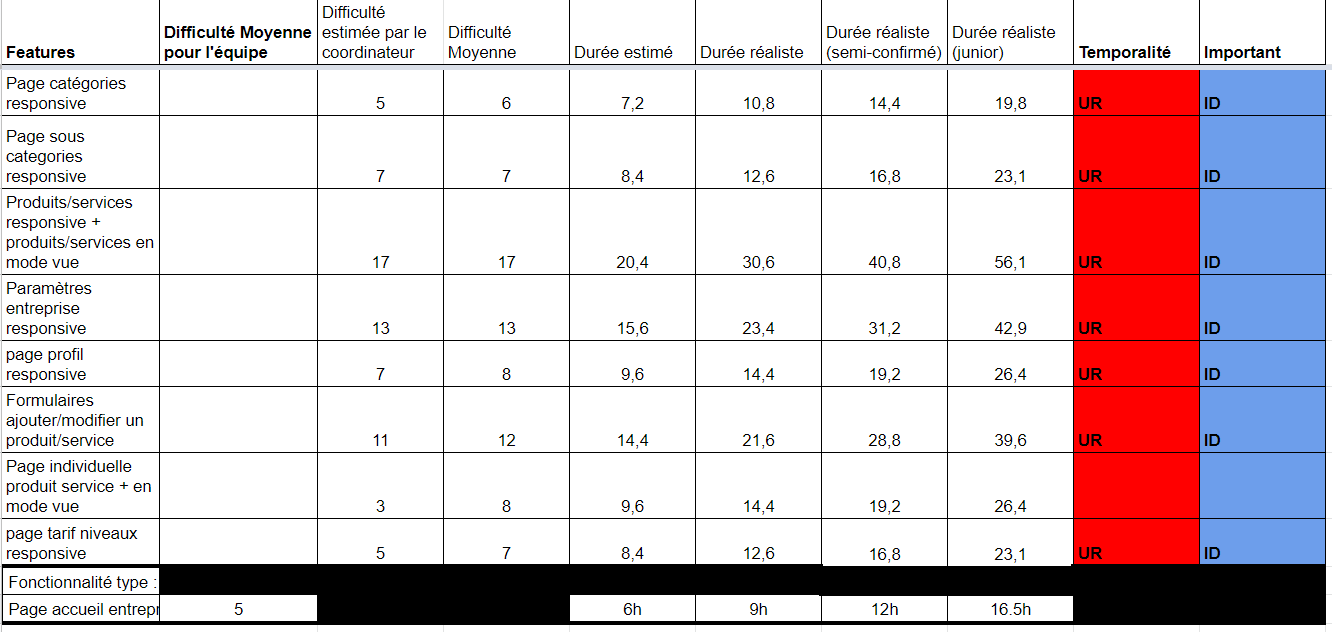
\includegraphics[width=\textwidth]{poker planning concret.png}
    \caption{Planning Poker de fin Novembre}
\end{figure}

Celui-ci était utilisé pour la planification et répartition du Responsive. 
Nous prenions une tâche de référence comparable, ici la page d'accueil entreprise en responsive, à laquelle une note et une durée estimée avaient été ajoutées.
Les durées réalistes sont calculées selon les majorations suivantes :

\begin{figure}[H]
    \centering
    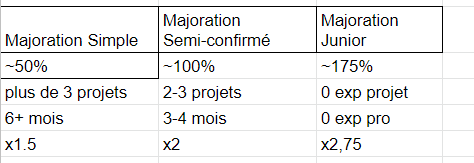
\includegraphics[width=10cm]{majoration pp.png}
\end{figure}

Pour les autres tâches, chaque membre assignait une difficulté à chacune relativement à celle de référence.

Et à partir de la difficulté moyenne de chaque tâche, on pouvait calculer leurs durées, proportionnellement aux durées/difficultés de la tâche de référence.

Ainsi, on pouvait assigner à chacun les tâches qui leur convenaient le mieux, en termes de difficulté et de compétences à développer, tout en faisant en sorte que cette répartition permette de respecter la deadline.


\subsubsection*{Journal de bord et Tableau des tâches}

Ces outils permettent de faciliter la rédaction des rapports et de garder un suivi des tâches à faire ou accomplies.\\

Le journal de bord comporte plusieurs onglets : Journalier, Hebdomadaire, Mensuel. 

\begin{figure}[H]
    \centering
    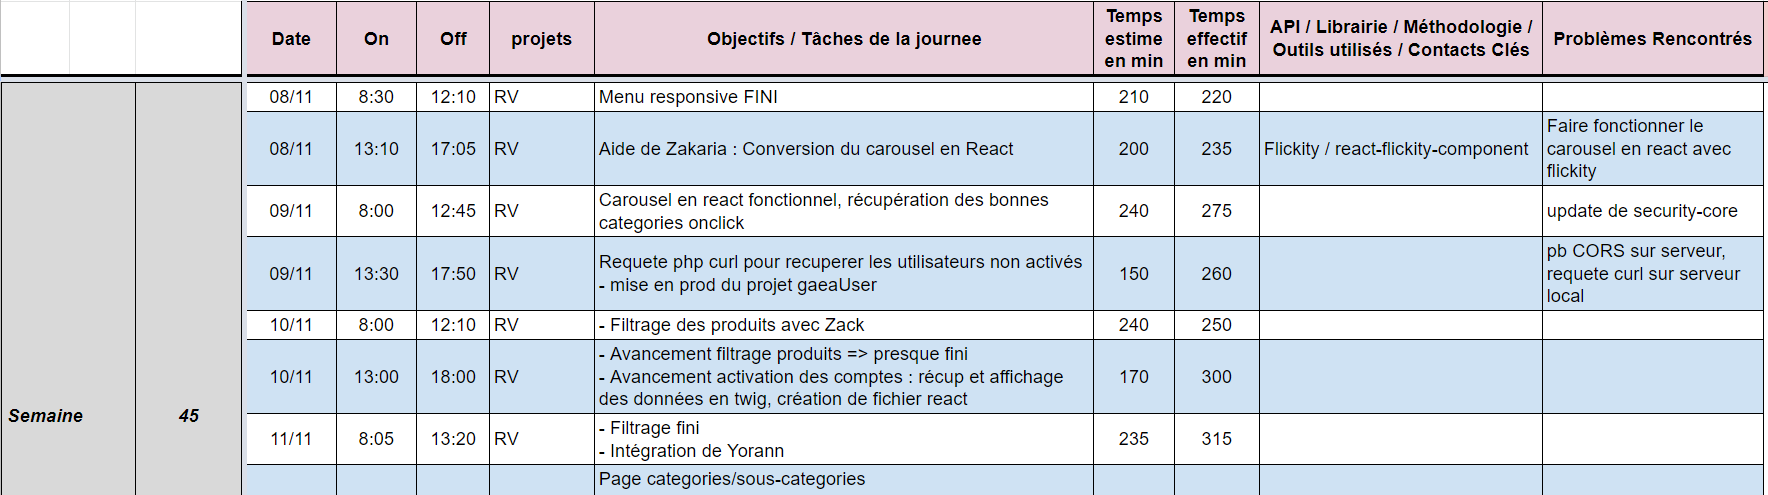
\includegraphics[width=\textwidth]{jdb.png}
    \caption{Extrait du journal de bord journalier}
\end{figure}

Les temps effectifs de la semaine sont additionnés et les heures effectuées sont répertoriées dans le Ga-Time :

\begin{figure}[H]
    \centering
    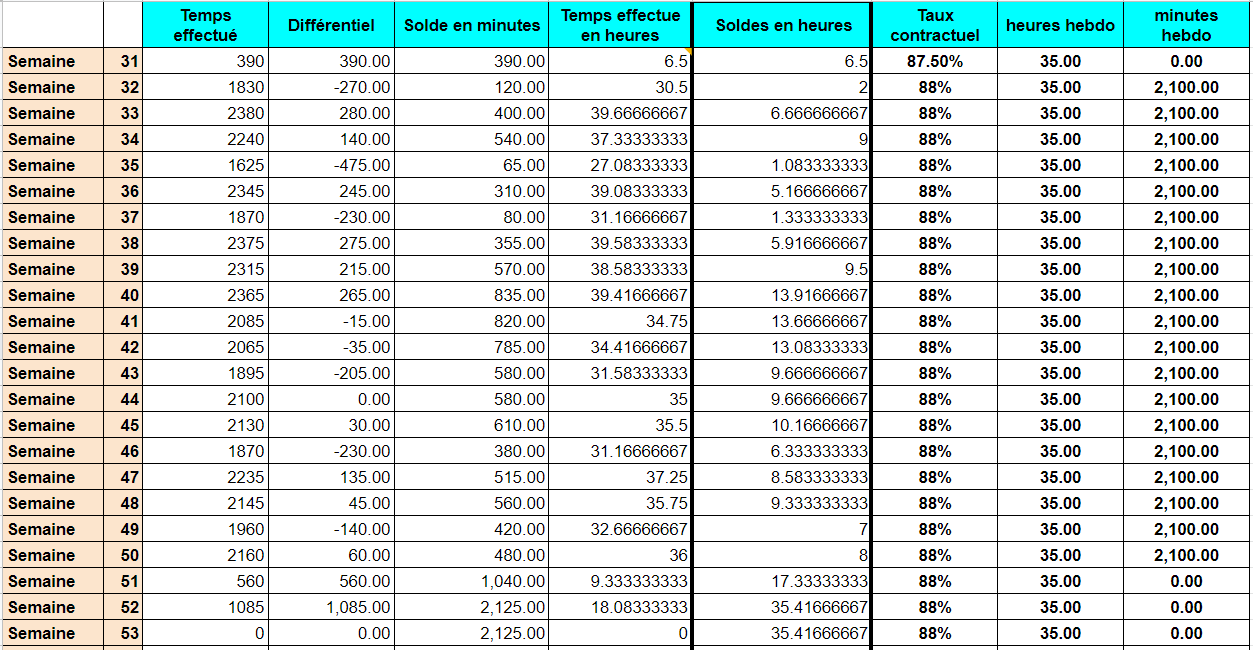
\includegraphics[width=\textwidth]{gatime.png}
\end{figure}

Le tableau des tâches permet de décomposer les tâches en sous-tâches et de pouvoir planifier le travail efficacement :

\begin{figure}[H]
    \centering
    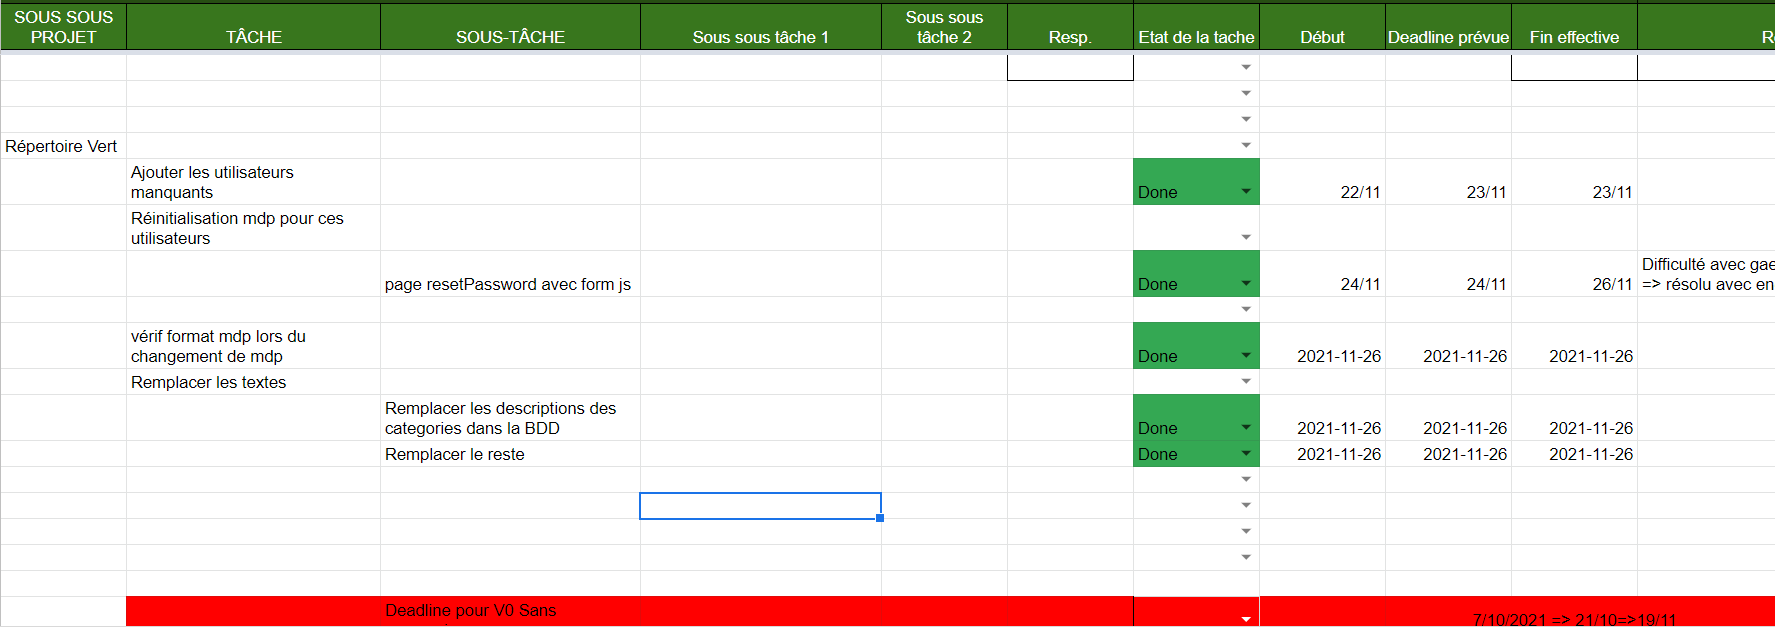
\includegraphics[width=\textwidth]{tableau_taches.png}
\end{figure}


% \label{longtab}

% On peut faire un tableau compliqué dans lequel je ne sais pas encore quoi mettre :

% \begin{table}[h!]
%     \begin{center}
%       \caption{Tableau avec booktabs}
%       \label{tab:beautifulTab}
%       \begin{tabular}{l|S|r}
%         \toprule % <-- Toprule here
%         \textbf{Value 1} & \textbf{Value 2} & \textbf{Value 3}\\
%         $\delta$ & $\theta$ & $\zeta$ \\
%         \midrule % <-- Midrule here
%         1 & 42 & a\\
%         2 & 75 & b\\
%         3 & 98 & c\\
%         \bottomrule % <-- Bottomrule here
%       \end{tabular}
%     \end{center}
%   \end{table}

% Et on peut aussi faire de longs tableaux qui vont sur plusieurs pages :

% \begin{longtable}{c|cc|cc}
%     \caption{Alice and Bob's bases and bits}
%     \label{tab:aeb}\\
%     \toprule
%           & \multicolumn{2}{c|}{\textbf{Alice}} & \multicolumn{2}{c}{\textbf{Bob}}                  \\
%     \midrule
%     Bit n° & Basis (+ or $\times$)      & Bit (0 or 1)            & Basis    & Bit \\ \hline
  
%     \endfirsthead % <-- This denotes the end of the header, which will be shown on the first page only
  
%     \toprule
%           & \multicolumn{2}{c|}{\textbf{Alice}} & \multicolumn{2}{c}{\textbf{Bob}}                  \\
%     \midrule
%     Bit n° & Basis (+ or $\times$)      & Bit (0 or 1)            & Basis    & Bit \\ \hline
%     $\vdots$ & $\vdots$                 & $\vdots$                & $\vdots$ & $\vdots$ \\
  
%     \endhead % <-- Everything between \endfirsthead and \endhead will be shown as a header on every page
%     $\vdots$ & $\vdots$                 & $\vdots$                & $\vdots$ & $\vdots$ \\
%     \endfoot % <-- Everything between \endhead and \endfoot will be shown as a footer on every page
%     \endlastfoot
%     1      & +                          & 1                       & +        & 1   \\
%     2      & +                          & 0                       & $\times$ & 1   \\
%     3      & +                          & 1                       & $\times$ & 0   \\
%     4      & $\times$                   & 1                       & +        & 1   \\
%     5      & $\times$                   & 1                       & +        & 1   \\
%     6      & $\times$                   & 1                       & +        & 0   \\
%     7      & +                          & 1                       & $\times$ & 0   \\
%     8      & +                          & 0                       & $\times$ & 1   \\
%     9      & +                          & 0                       & $\times$ & 0   \\
%     10     & $\times$                   & 1                       & $\times$ & 0   \\
%     11     & +                          & 1                       & +        & 1   \\
%     12     & +                          & 1                       & +        & 1   \\
%     13     & $\times$                   & 0                       & $\times$ & 0   \\
%     14     & $\times$                   & 0                       & $\times$ & 0   \\
%     15     & $\times$                   & 0                       & $\times$ & 0   \\
%     16     & $\times$                   & 1                       & +        & 1   \\
%     17     & +                          & 1                       & +        & 1   \\
%     18     & +                          & 0                       & +        & 0   \\
%     19     & +                          & 0                       & $\times$ & 0   \\
%     20     & +                          & 1                       & $\times$ & 0   \\
%     21     & +                          & 1                       & $\times$ & 1   \\
%     22     & +                          & 1                       & +        & 1   \\
%     23     & $\times$                   & 1                       & +        & 1   \\
%     24     & $\times$                   & 1                       & $\times$ & 1   \\
%     25     & $\times$                   & 0                       & $\times$ & 0   \\
%     26     & +                          & 0                       & $\times$ & 1   \\
%     27     & +                          & 1                       & +        & 1   \\
%     28     & +                          & 1                       & $\times$ & 1   \\
%     29     & +                          & 0                       & $\times$ & 0   \\
%     30     & +                          & 0                       & $\times$ & 1   \\
%     31     & +                          & 0                       & +        & 0   \\
%     32     & +                          & 0                       & +        & 0   \\
%     33     & +                          & 1                       & +        & 1   \\
%     34     & $\times$                   & 1                       & $\times$ & 1   \\
%     35     & $\times$                   & 0                       & $\times$ & 0   \\
%     36     & $\times$                   & 0                       & $\times$ & 0   \\
%     37     & $\times$                   & 1                       & +        & 0   \\
%     38     & $\times$                   & 1                       & +        & 0   \\
%     39     & +                          & 1                       & +        & 1   \\
%     40     & +                          & 0                       & $\times$ & 0   \\
%     41     & +                          & 0                       & $\times$ & 0   \\
%     42     & $\times$                   & 0                       & $\times$ & 0   \\
%     43     & $\times$                   & 1                       & +        & 1   \\
%     44     & +                          & 1                       & +        & 1   \\
%     45     & $\times$                   & 1                       & +        & 0   \\
%     46     & $\times$                   & 0                       & +        & 0   \\
%     47     & +                          & 0                       & $\times$ & 1   \\
%     48     & +                          & 1                       & +        & 1   \\
%     49     & $\times$                   & 1                       & +        & 0   \\
%     50     & +                          & 0                       & +        & 0   \\
%     51     & +                          & 1                       & $\times$ & 1   \\
%     52     & $\times$                   & 0                       & $\times$ & 0   \\ \hline
%     \bottomrule
%   \end{longtable}

% Si vous vous demandez la différence entre \incode{toprule} et \incode{hline} : \shortUrl{https://tex.stackexchange.com/questions/156122/booktabs-what-is-the-difference-between-toprule-and-hline}